\chapter{Threat Model} \label{ch:threat-model}
\section{Assets}
As part of the thread modelling phase, assets of the system were identified. These can be found in table \ref{tb:assets}.
\begin{table}[!ht]
    \centering
    \begin{tabular}{r l}
        \hline
        \textbf{ID} & \textbf{Description} \\ \hline
        1  & Blah        \\
        2  & Bleh        \\
        3  & Bloh        \\ \hline
    \end{tabular}
    \caption{The identified assets of the system}
    \label{tb:assets}
\end{table}

\section{Overview of the System Architecture}
\begin{figure}[!ht]
  \begin{center}
    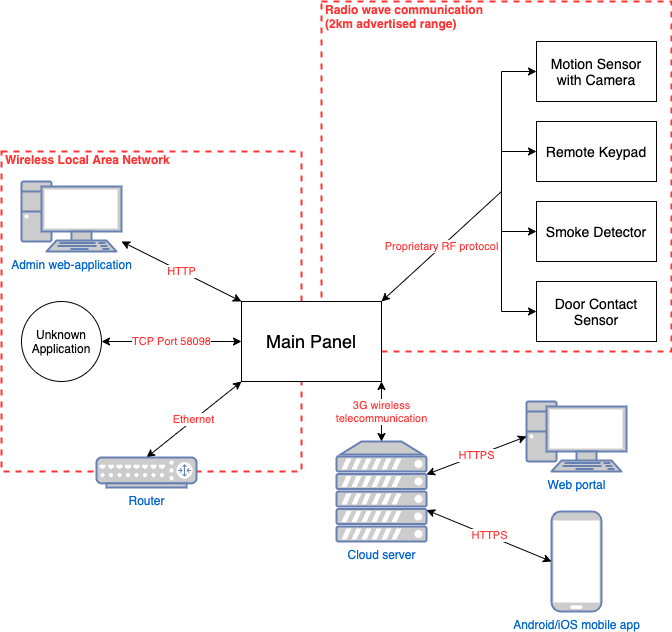
\includegraphics[width=\textwidth]{images/system-overview.png}
  \end{center}
  \caption{Overview of the System Architecture}
  \label{fig:system-overview}
\end{figure}